\section{Estrategia de búsqueda usando bola de nieve}\label{sec:bola-de-nieve}

En esta etapa, la estrategia de snowballing se aplicó a la totalidad de los 18 estudios elegidos (17 mediante el proceso de selección y uno incluido directamente), en lugar de limitarse a un grupo reducido de artículos semilla. Esta decisión amplió la cobertura de la revisión y redujo el riesgo de omitir literatura relevante, fortaleciendo la exhaustividad del protocolo.

En este proceso se aplicaron las estrategias de bola de nieve directa \textit{(forward)} e inversa \textit{(backward)}, con el objetivo de identificar literatura adicional relevante que no hubiera sido recuperada durante la búsqueda automática en las bases de datos. La búsqueda por bola de nieve inversa permitió identificar un estudio adicional, mientras que la búsqueda por bola de nieve directa permitió identificar tres estudios adicionales, lo que resultó en un total de cuatro estudios incorporados.

El resumen de este proceso puede observarse en la \autoref{fig:proceso-snowball}.

\begin{figure}[H]
	\begin{center}
		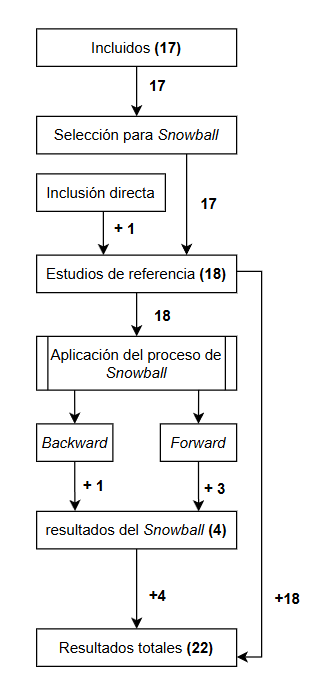
\includegraphics[width=0.4\textwidth]{mainmatter/II-desarrollo-metodologico/sms/imagenes/proceso-snowball.png}
	\end{center}
	\caption{Resumen del proceso de búsqueda por bola de nieve}
	\label{fig:proceso-snowball}
\end{figure}
